\documentclass[fleqn]{article}
\oddsidemargin 0.0in
\textwidth 6.0in
\thispagestyle{empty}
\usepackage{import}
\usepackage{amsmath}
\usepackage{graphicx}
\usepackage{flexisym}
\usepackage{calligra}
\usepackage{amssymb}
\usepackage{bigints} 
\usepackage[english]{babel}
\usepackage[utf8x]{inputenc}
\usepackage{float}
\usepackage[colorinlistoftodos]{todonotes}


\DeclareMathAlphabet{\mathcalligra}{T1}{calligra}{m}{n}
\DeclareFontShape{T1}{calligra}{m}{n}{<->s*[2.2]callig15}{}
\newcommand{\scriptr}{\mathcalligra{r}\,}
\newcommand{\boldscriptr}{\pmb{\mathcalligra{r}}\,}

\definecolor{hwColor}{HTML}{1a0252}

\begin{document}

  \begin{titlepage}

    \newcommand{\HRule}{\rule{\linewidth}{0.5mm}}

    \center


    \textsc{\LARGE Arizona State University}\\[1.5cm]

    \textsc{\LARGE Quantum Physics II}\\[1.5cm]


    \begin{figure}
      
\includegraphics[width=\linewidth]{asu.png}
    \end{figure}


    \HRule \\[0.4cm]
    { \huge \bfseries Problem Set 2}\\[0.4cm] 
    \HRule \\[1.5cm]

    \textbf{Behnam Amiri}

    \bigbreak

    \textbf{Prof: Onur Erten}

    \bigbreak


    \textbf{{\large \today}\\[2cm]}

    \vfill

  \end{titlepage}

  \begin{enumerate}
    \item \textbf{4-16} A rod of proper length $l_0$ is at rest in a frame $S^'$. It lies in the $(x^',y^')$ plane and makes
    an angle of $sin^{-1}(\dfrac{3}{5})$ with the $x^'$ axis. If $S^'$ moves with constant velocity $v$ parallel to the 
    $x$ axis of another frame $S:$
    \begin{enumerate}
      \item What must be the value of $v$ if, as measured in $S$, the rod is at $45^\circ$ to the $x$ axis?

        \textcolor{hwColor}{
          $
            \theta=sin^{-1}(\dfrac{3}{5})
            \\
            \\
            \begin{cases}
              l_x=l_0 cos(45^{\circ}) 
              \\
              \\
              l^'_x=l_0 cos(\theta)
            \end{cases}
            \\
            \\
            \\
            l_x=l^'_x \sqrt{1-\left(\dfrac{v}{c}\right)^2}
            \\
            \\
            \\
            \left(\dfrac{l_x}{l^'_x}\right)^2=1-\left(\dfrac{v}{c}\right)^2
            \\
            \\
            \\
            \left(\dfrac{v}{c}\right)^2=1-\left(\dfrac{l_x}{l^'_x}\right)^2
            \\
            \\
            \\
            v^2=c^2\left[1-\left(\dfrac{l_x}{l^'_x}\right)^2\right]
            =c^2\left[1-\left(\dfrac{l_0 cos(45^{\circ})}{l_0 cos(\theta)}\right)^2\right]
            =c^2\left[1-\left(\dfrac{cos(45^{\circ})}{cos(\theta)}\right)^2\right]
            \\
            \\
            \\
            \therefore ~~~ v \approx 1.40 \times 10^{8} ~~~ \checkmark
          $
        }


      \item What is the length of the rod as measured in $S$ under these conditions?


        \textcolor{hwColor}{
          $
            l=\dfrac{l_0}{\sqrt{1-\left(\dfrac{v}{c}\right)^2}}
            \\
            \\
            \\
            \therefore ~~~~ l=1.14 l_0 ~~~ \checkmark
          $
        }

    \end{enumerate}


    \item \textbf{5-7} An inertial system $S_1$ has a constant velocity $v_1$ along the $x$ axis relative to an inertial system $S$.
    Inertial system $S_2$ has a velocity $v_2$ relative to $S_1$. Two successive Lorentz-Einstein transformations enable us to
    go from $(x, y, z, t)$ to $(x_1, y_1, z_1, t_1)$ and then from $(x_1, y_1, z_1, t_1)$ to $(x_2, y_2, z_2, t_2)$. Show that 
    this gives the same result as a single Lorentz-Einstein transformation from $(x, y, z, t)$ to $(x_2, y_2, z_2, t_2)$,
    provided we take the velocity $v$ of $S_2$ relative to $S$ as
    $$v=\dfrac{v_1+v_2}{1+\dfrac{v_1 v_2}{c^2}}$$


    \item \textbf{5-9} Three identical radio transmitters $A, B,$ and $C,$ each transmitting at the frequency $v_0$ in its own
    rest frame, are in motion as shown.

    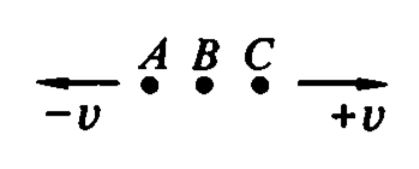
\includegraphics[height=3cm, width=4cm]{1.JPG}

    \begin{enumerate}
      \item What is the frequency of $B^'$s signals as received by $C$?
      
        \textcolor{hwColor}{
          $
            \\
            v=v_0 \sqrt{\dfrac{1-\left(\dfrac{v}{c}\right)}{1+\left(\dfrac{v}{c}\right)}}
            \\
          $
        }


      \item What is the frequency of $A^'$s signals as received by $C$?

        \textcolor{hwColor}{
          $
            \\
            v=v_0 \sqrt{\dfrac{1-\left(\dfrac{v}{c}\right)}{1+\left(\dfrac{v}{c}\right)}} \sqrt{\dfrac{1-\left(\dfrac{v}{c}\right)}{1+\left(\dfrac{v}{c}\right)}}
            \\
            \\
            \\
            \therefore ~~~~ v=v_0 \dfrac{1-\left(\dfrac{v}{c}\right)}{1+\left(\dfrac{v}{c}\right)} ~~~ \checkmark
            \\
          $
        }

    \end{enumerate}


  \end{enumerate}

\end{document}